\documentclass[12pt]{article}
\usepackage[english]{babel}
\usepackage[utf8]{inputenc}
\usepackage [autostyle, english = american]{csquotes}
%\MakeOuterQuote{"}
\usepackage{url}
\usepackage{import}
\usepackage{tabularx}
\usepackage{booktabs}
\usepackage{amsmath}
\usepackage{amsfonts}
\usepackage{mathcomp}
\usepackage{graphicx}
\usepackage[margin=1.25in]{geometry}
\usepackage{caption}
\usepackage{multirow}
\usepackage[table]{xcolor}
\usepackage{rotating}
\usepackage{mathtools}
\usepackage{xr}
\usepackage{breakcites}
\usepackage[]{mcode}
\usepackage{matlab-prettifier}
\usepackage{listings} %For code in appendix
\usepackage{color} %red, green, blue, yellow, cyan, magenta, black, white
\definecolor{mygreen}{RGB}{28,172,0} % color values Red, Green, Blue
\definecolor{mylilas}{RGB}{170,55,241}
\usepackage{gensymb}
\usepackage{makeidx}
\makeindex
\pagestyle{empty}
\usepackage{endnotes}
\usepackage{lineno}
%\linenumbers
\begin{document}

%%%%For color MATLAB Scripts
\lstset
{ %Formatting for code in appendix
    language=Matlab,
    basicstyle=\scriptsize,
    numbers=left,
    stepnumber=1,
    showstringspaces=false,
    tabsize=1,
    breaklines=true,
    breakatwhitespace=false,
}

{\bf \flushleft Simulation of  a Smart-Navigated UAV Disaster Response Fleet} 
\small
\\OVERLEAF PROJECT: https://www.overleaf.com/read/tmspxpmbxnst
% \vspace{.1in}

% {\flushleft \small
% {\bf 
% Paul Isihara\\
% with\\
% Christy Baars\\
% Steven Kwon\\
% William McKinnon\\
% Joseph Nussbaum\\
% Carrie Steggerda\\
% Joyce Yan}\\
% Wheaton College}

% \vspace{.2in}

\vspace{.2in}
{\small Although unmanned aerial vehicles (UAVs) have proven to be useful in disaster response, OCHA has asserted that until their usage becomes more prevalent in daily civilian life, the risks in full-scale deployment of UAVs in disaster response must first be reduced by careful development of best practice standards. Simulation modeling and analysis of disaster response UAV fleets is a timely and important part of this development process. Difficulties in humanitarian logistics in Puerto Rico after Hurricane Maria (2017) give specific context for designing a general purpose simulation model of a  smart-navigated UAV disaster response fleet. }

\newpage
{\flushleft TASKS}

{\flushleft 1.}  Modify the script UAVStep1.m to add a 3rd base and lo-speed UAV just north of San Lucas Hospital.


{\flushleft 2.} Create a class requestManager.m which has properties ID number,  time, location and priority (hi or lo) of a request for help, and a method which plots the location of the request, ID number color coded by priority (red=hi, blue=lo).  Create a hi priority request near Utuado and a lo priority request near Aibonito.  

\newpage
\begin{figure}[!htpb]  
\centering
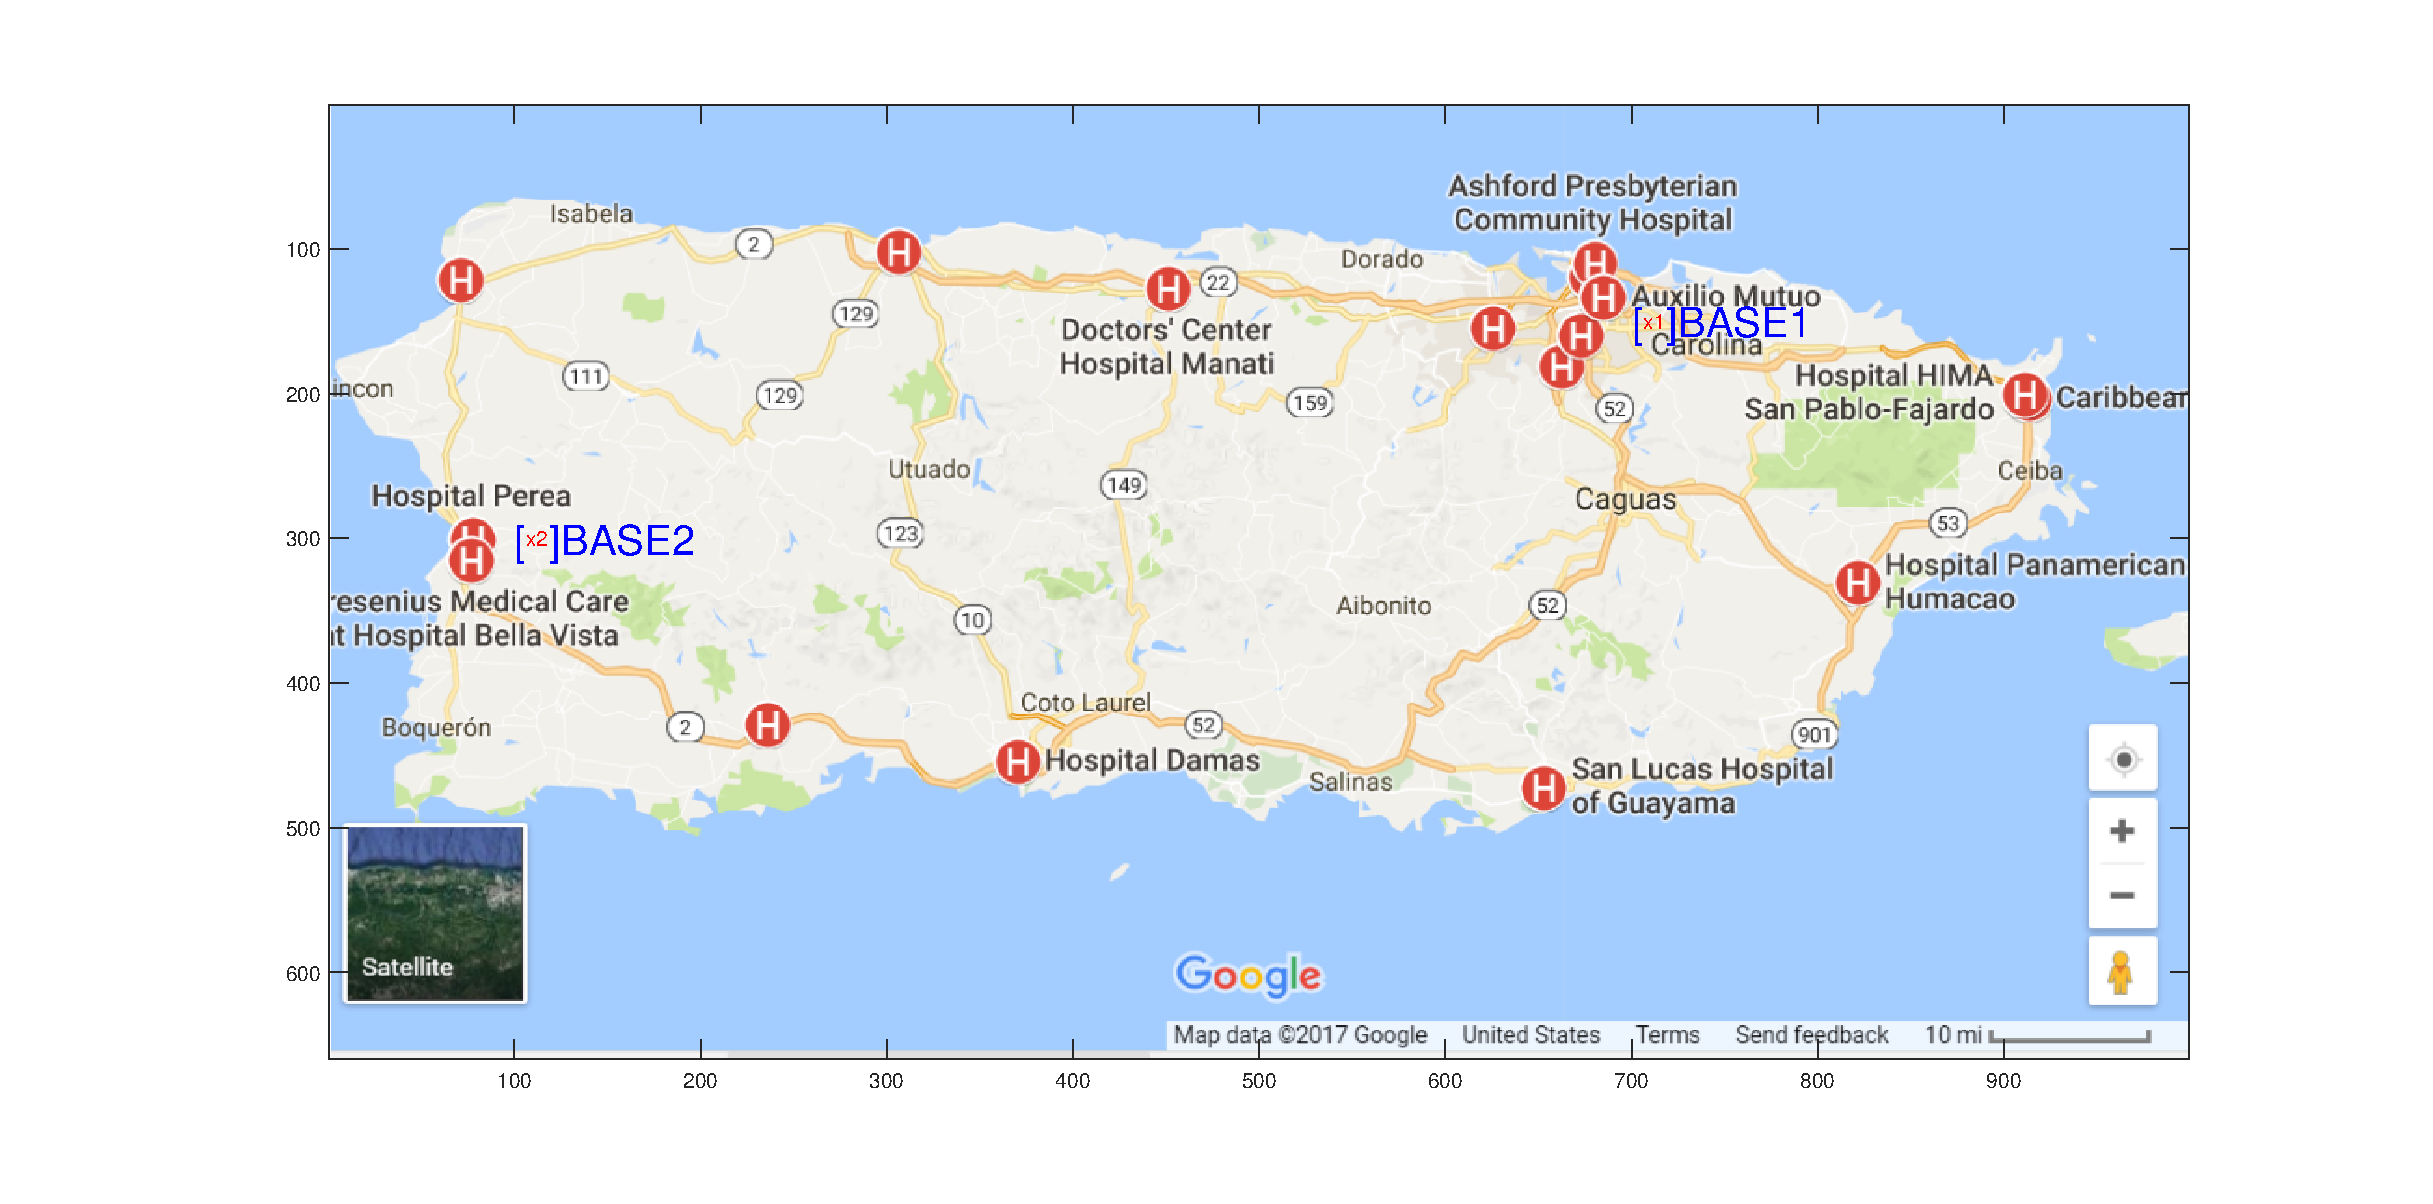
\includegraphics[width=6.25in, height=5in]{fig1.eps}
\caption{Output of UAVStep1.m shows UAV home basis.}
\label{fig8}
\end{figure}



\begin{table}[!htpb]
\centering
\begin{tabular}{|l|}\hline
The Main Script UAVStep1.m \\
\parbox[b]{6.2in}{\lstinputlisting[style=Matlab-editor,firstline=1, lastline=37, firstnumber=1]{UAVStep1.m}}\\\hline
\end{tabular}
\end{table}
\begin{table}[!htpb]
\centering
\begin{tabular}{|l|}\hline
The Class fleetManager.m \\
\parbox[b]{6.2in}{\lstinputlisting[style=Matlab-editor,firstline=1, lastline=30, firstnumber=1]{fleetManager.m}}\\\hline
\end{tabular}
\end{table}


\end{document}